\documentclass[tikz]{standalone}
\usepackage{tikz}
\usepackage{amsmath}
\usepackage{amsfonts}

\newcommand{\manifold}[1][M]{\mathcal{#1}}
\newcommand{\tvec}[2]{\left(\partial\indices{_{#1}}\right)_{#2}}
\newcommand{\tfld}[1]{\partial\indices{_{#1}}}
\newcommand{\lder}[1]{\mathcal{L}_{#1}}
\newcommand{\alt}[2]{\Lambda^{#1}(\manifold[#2])}
\newcommand{\bnd}[1]{\partial\manifold[#1]}
\newcommand{\irrshape}[3]{% r, dr, sample
    \draw plot 
        [smooth cycle, samples=#3, domain={1:#3}] 
        ({(\x*360/#3+8*(2*rnd-1))}:{#1+#2*(2*rnd-1)})
}
\DeclareMathOperator{\idd}{id}
\DeclareMathOperator{\sgn}{sgn}

\begin{document}
    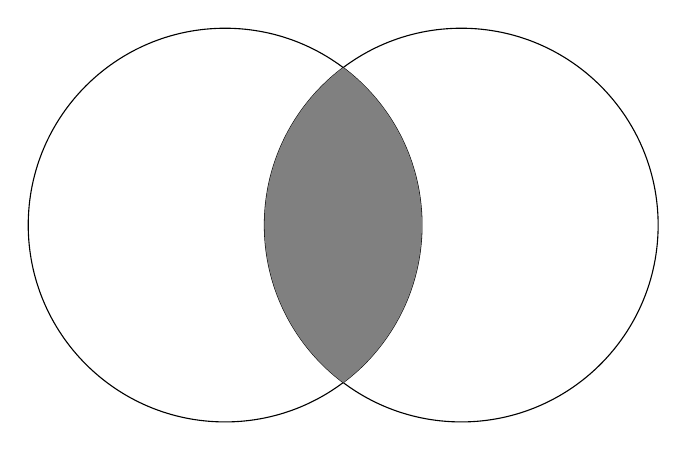
\begin{tikzpicture}[scale=0.5]
        \draw (-3, 0) circle (5);
        \draw (3, 0) circle (5);
        \begin{scope}
            \clip (-3, 0) circle (5);
            \fill[gray] (3, 0) circle (5);
        \end{scope}
    \end{tikzpicture}
\end{document}